\section{57 - MAT - WS 4.1, AN 3.3 - Überraschungseier - Matura 2014/15 2. Nebentermin}

\begin{langesbeispiel} \item[0] %PUNKTE DES BEISPIELS
	
Ein italienischer Süßwarenhersteller erzeugt das Produkt Kinder Überraschung (auch als "`Überraschungsei"' bekannt). Das Ei soll aus 20\,g Schokolade bestehen. Im Inneren des Eies befindet sich in einer gelben Kapsel ein Spielzeug. Diese Kapsel hat näherungsweise die Form eines Drehzylinders, auf dessen Grund- und Deckfläche Halbkugeln aufgesetzt werden. Das Volumen der Kapsel beträgt ungefähr 36\,cm$^3$ und deren Oberfläche 55\,cm$^2$.

\begin{center}
	\resizebox{0.8\linewidth}{!}{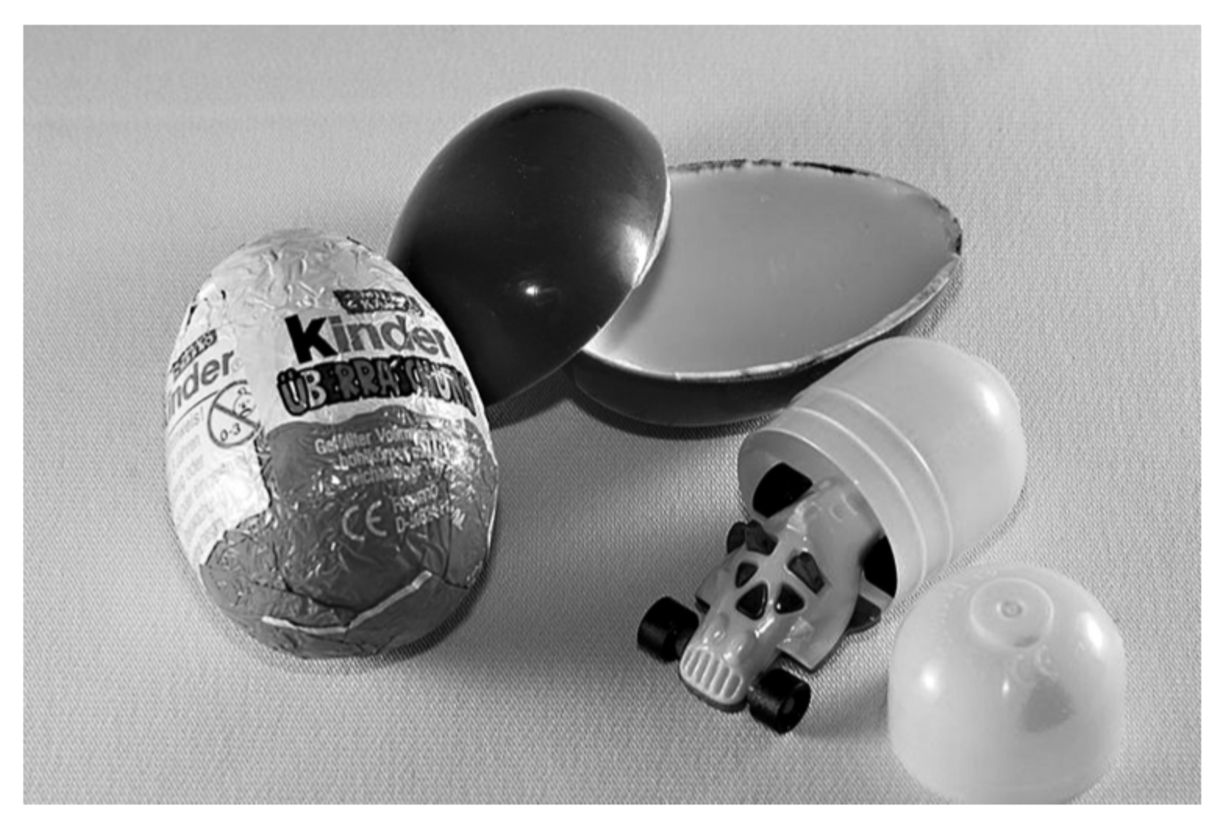
\includegraphics{../_database/Bilder/Bild57-1.eps}}
\end{center}
\begin{scriptsize}\begin{singlespace}Bildquelle: https://de.wikipedia.org/wiki/Datei:Überraschungsei.jpg [01.06.2015] (Urheber: A. Kniesel, Lizenz: CC BY-SA 3.0)\end{singlespace}\end{scriptsize}

\subsection{Aufgabenstellung:}
\begin{enumerate}
	\item Bei der Qualitätskontrolle gelten Schokoladeneier, deren Masse um mehr als 0,5\,g vom Sollwert 20\,g abweichen, als Ausschuss. Bei einer Kontrolle wurden nach dem Zufallsprinzip 500 Schokoladeneier einer Produktionsserie ausgewählt und überprüft. Dabei wurden 15 als Ausschuss aussortiert.\leer
	
 Gib ein symmetrisches 90-\%-Konfidenzintervall für den relativen Anteil $p$ an Ausschusseiern in der gesamten Produktionsserie an!\leer

 Gib an, durch welche Maßnahme man die Breite des Konfidenzintervalls bei vorgegebenem Konfidenzniveau (Sicherheit) verringern kann!\leer

\item Der Hersteller überlegt, die gelbe Kapsel in Zukunft nur in Form eines Drehzylinders ohne aufgesetzte Halbkugeln zu produzieren. Das Volumen $V$ der Kapsel soll dabei unverändert bleiben, ebenso wie die Form des Schokoladeneies. Die Oberfläche $O(r)$ des angedachten Drehzylinders kann in Abhängigkeit vom Radius $r$ durch die Funktion $O$ mit der Gleichung $O(r)=2r^2\pi+2\cdot V\cdot r^{-1}$ beschrieben werden. Der Radius $r$ darf dabei nur Werte im Bereich $(0\,cm; 1,9\,cm]$ annehmen, damit der Zylinder in das Schokoladenei passt.\leer

 Berechne die minimal mögliche Oberfläche der geplanten zylindrischen Kapsel!\leer

 Weise durch Differenzialrechnung nach, dass an der berechneten Stelle tatsächlich ein Minimum vorliegt!
						\end{enumerate}\leer
				
\antwort{
\begin{enumerate}
	\item \subsection{Lösungserwartung:} 
	
$h=0,03$

$0,03\,\pm\,1,645\cdot\sqrt{\frac{0,03\cdot(1-0,03)}{500}} \approx 0,03\,\pm\,0,013 \Rightarrow [0,017;0,043]$\leer

Mögliche Maßnahme:

Durch eine Erhöhung der Anzahl der kontrollierten Schokoladeneier auf mehr als 500 kann eine Verringerung der Breite des Konfidenzintervalls erreicht werden.
		
	\subsection{Lösungsschlüssel:}
	\begin{itemize}
		\item Ein Punkt für ein korrektes Intervall. Andere Schreibweisen des Ergebnisses (als Bruch oder Dezimalzahl) sind ebenfalls als richtig zu werten. 
		
		Toleranzintervall für den unteren Wert: $[0,017; 0,02]$ 
		
		Toleranzintervall für den oberen Wert: $[0,042; 0,05]$ 
		
		Die Aufgabe ist auch dann als richtig gelöst zu werten, wenn bei korrektem Ansatz das Ergebnis aufgrund eines Rechenfehlers nicht richtig ist. 
		\item Ein Punkt für eine (sinngemäß) korrekte Angabe der entsprechenden Änderung. Andere angeführte korrekte Maßnahmen sind ebenfalls als richtig zu werten.
	\end{itemize}
	
	\item \subsection{Lösungserwartung:}
			
			$O'(r)=4r\pi-72\cdot r^{-2}=4r\pi-\frac{72}{r^2}$
	
	$4r\pi-\frac{72}{r^2}=0$
	
	$r^3=\frac{18}{\pi}$
	
	$r=\sqrt[3]{\frac{18}{\pi}} \Rightarrow r\approx 1,79$\,cm
	
	$O(1,79)\approx 60,4$\,cm$^2$
	
	$O''(r)=4\pi+144\cdot r^{-3}=4\pi+\frac{144}{r^3}$
	
	$O''(1,79)\approx 37,7>0$, daher liegt ein lokales Maximum vor.

	\subsection{Lösungsschlüssel:}
	
\begin{itemize}
	\item    Ein Punkt für eine korrekte Berechnung der minimalen Oberfläche, wobei die Einheit "`cm$^2$"' nicht angeführt sein muss. 
	
	Toleranzintervall: $[60\,\text{cm}^2; 61\,\text{cm}^2] $ 
	
	Die Aufgabe ist auch dann als richtig gelöst zu werten, wenn bei korrektem Ansatz das Ergebnis aufgrund eines Rechenfehlers nicht richtig ist. 
	\item  Ein Punkt für einen korrekten Nachweis. Andere angeführte korrekte Nachweise sind ebenfalls als richtig zu werten. 
\end{itemize}

\end{enumerate}}
		\end{langesbeispiel}